
\section{Motivation}

There are many research try to improve code completion using AST information \cite{izadi2022codefill} \cite{li2017code} \cite{kim2021code}. Because they would like the model to learn the syntactical structures. However, there are some drawbacks using AST in code completion. First, AST could create additional overhead and dependencies \cite{svyatkovskiy2020intellicode}. Second, to correctly retrieve the AST, the code need to be syntactically correct and complete. But code completion in practice, the code is incomplete and is tend to be unable to parse to AST. 

Therefore inspired by AST, we propose to use standard type information. Since the standard type information maintains the syntactical information, able to retrieve at any points with minimum false representations, and easy to use along the source code. The examples compare between AST parser results and standard type results are shown in Fig. \ref{fig:ASTvsType}. Thus, the standard type prediction is the auxiliary task in this paper.

\begin{figure}
    \centering
    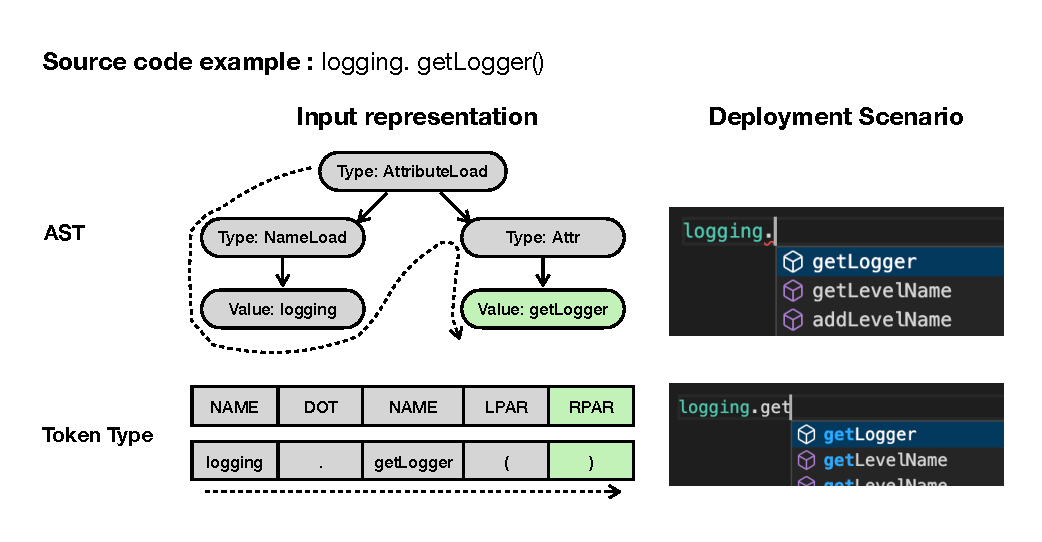
\includegraphics[width=\columnwidth]{figures/motivation.png}
    \caption{a) source code example for parsing. b) AST parsing result c) standard token types result}
    \label{fig:ASTvsType}
\end{figure}

